\chapter{Construcción Paralela de Redes Porosas Sujeta a $RG$}
\label{champ:PBSGR}
\bigskip
\barra
\bigskip
En este capítulo se describe la implementación paralela de los algoritmos descritos en el capítulo \ref{champ:BSGR} para la creación 
de redes porosas sujetas a Restricciones Geométricas. Las implementaciones paralelas trabajan sobre el modelo  de memoria compartida,
donde varios hilos cooperan en la construcción de una red porosa válida siguiendo los principales pasos de los algoritmos presentados en 
el capítulo anterior. El primer paso para las dos soluciones paralelas es la distribución espacial de la red entre los hilos a utilizar 
dicha distribución es igual para ambos algoritmos. Después de la distribuci\'on espacial de red cada algoritmo comenzara con su 
respectivo procedimiento de construcci\'on (inicializaci\'on, eliminaci\'on de violaciones y mejoramiento de la isotrop\'ia) en paralelo.
Primero presentaremos el algoritmo com\'un de distribución espacial y luego la paralelizaci\'on de las etapas de construcci\'on.

\section{Distribución Dinámica de la Red Porosa}
\label{sec:pdistribution}
En este paso una red porosa es dividida en $N$ subredes donde $N$ es el número de hilos a utilizar. El objetivo es dividir 
la red en $N$ partes las cuales deben mantener una estructura lo más parecida a un cubo; para lograr esto la red se divide a lo largo 
de los tres ejes $x$,$y$ y $z$ en $a$, $b$, y $c$ partes, respectivamente. Se debe cumplir que el producto de  $a$, $b$, y $c$ es igual 
a $N$. El tamaño de cada subred esta definido por $L_x \cdot L_y \cdot L_z$, como se puede observar en la Figura \ref{fig:distribution}. 
Por ejemplo, si tomamos $N=4$, una configuración generada ser\'ia $a=1,b=2,c=2$, mientras que para $N=45$ una configuración generada 
ser\'ia $a=3,b=3,c=5$, y para  $N = 27$ una configuración generada ser\'ia $a=3,b=3,c=3$, que representa la raíz cubica de 27. La mejor 
distribución se da cuando $a$, $b$, y $c$ corresponden a la raíz cubica de $N$; de esta forma las subredes generadas adoptan
una estructura cúbica que ayuda a que la distribución de los poros sea equitativa a lo largo de los ejes $x$, $y$ y $z$ de cada subred.
En la Figura \ref{fig:particionamiento} se muestran algunos ejemplos de particionamiento.\\

\begin{figure}[hbtp]
\centering
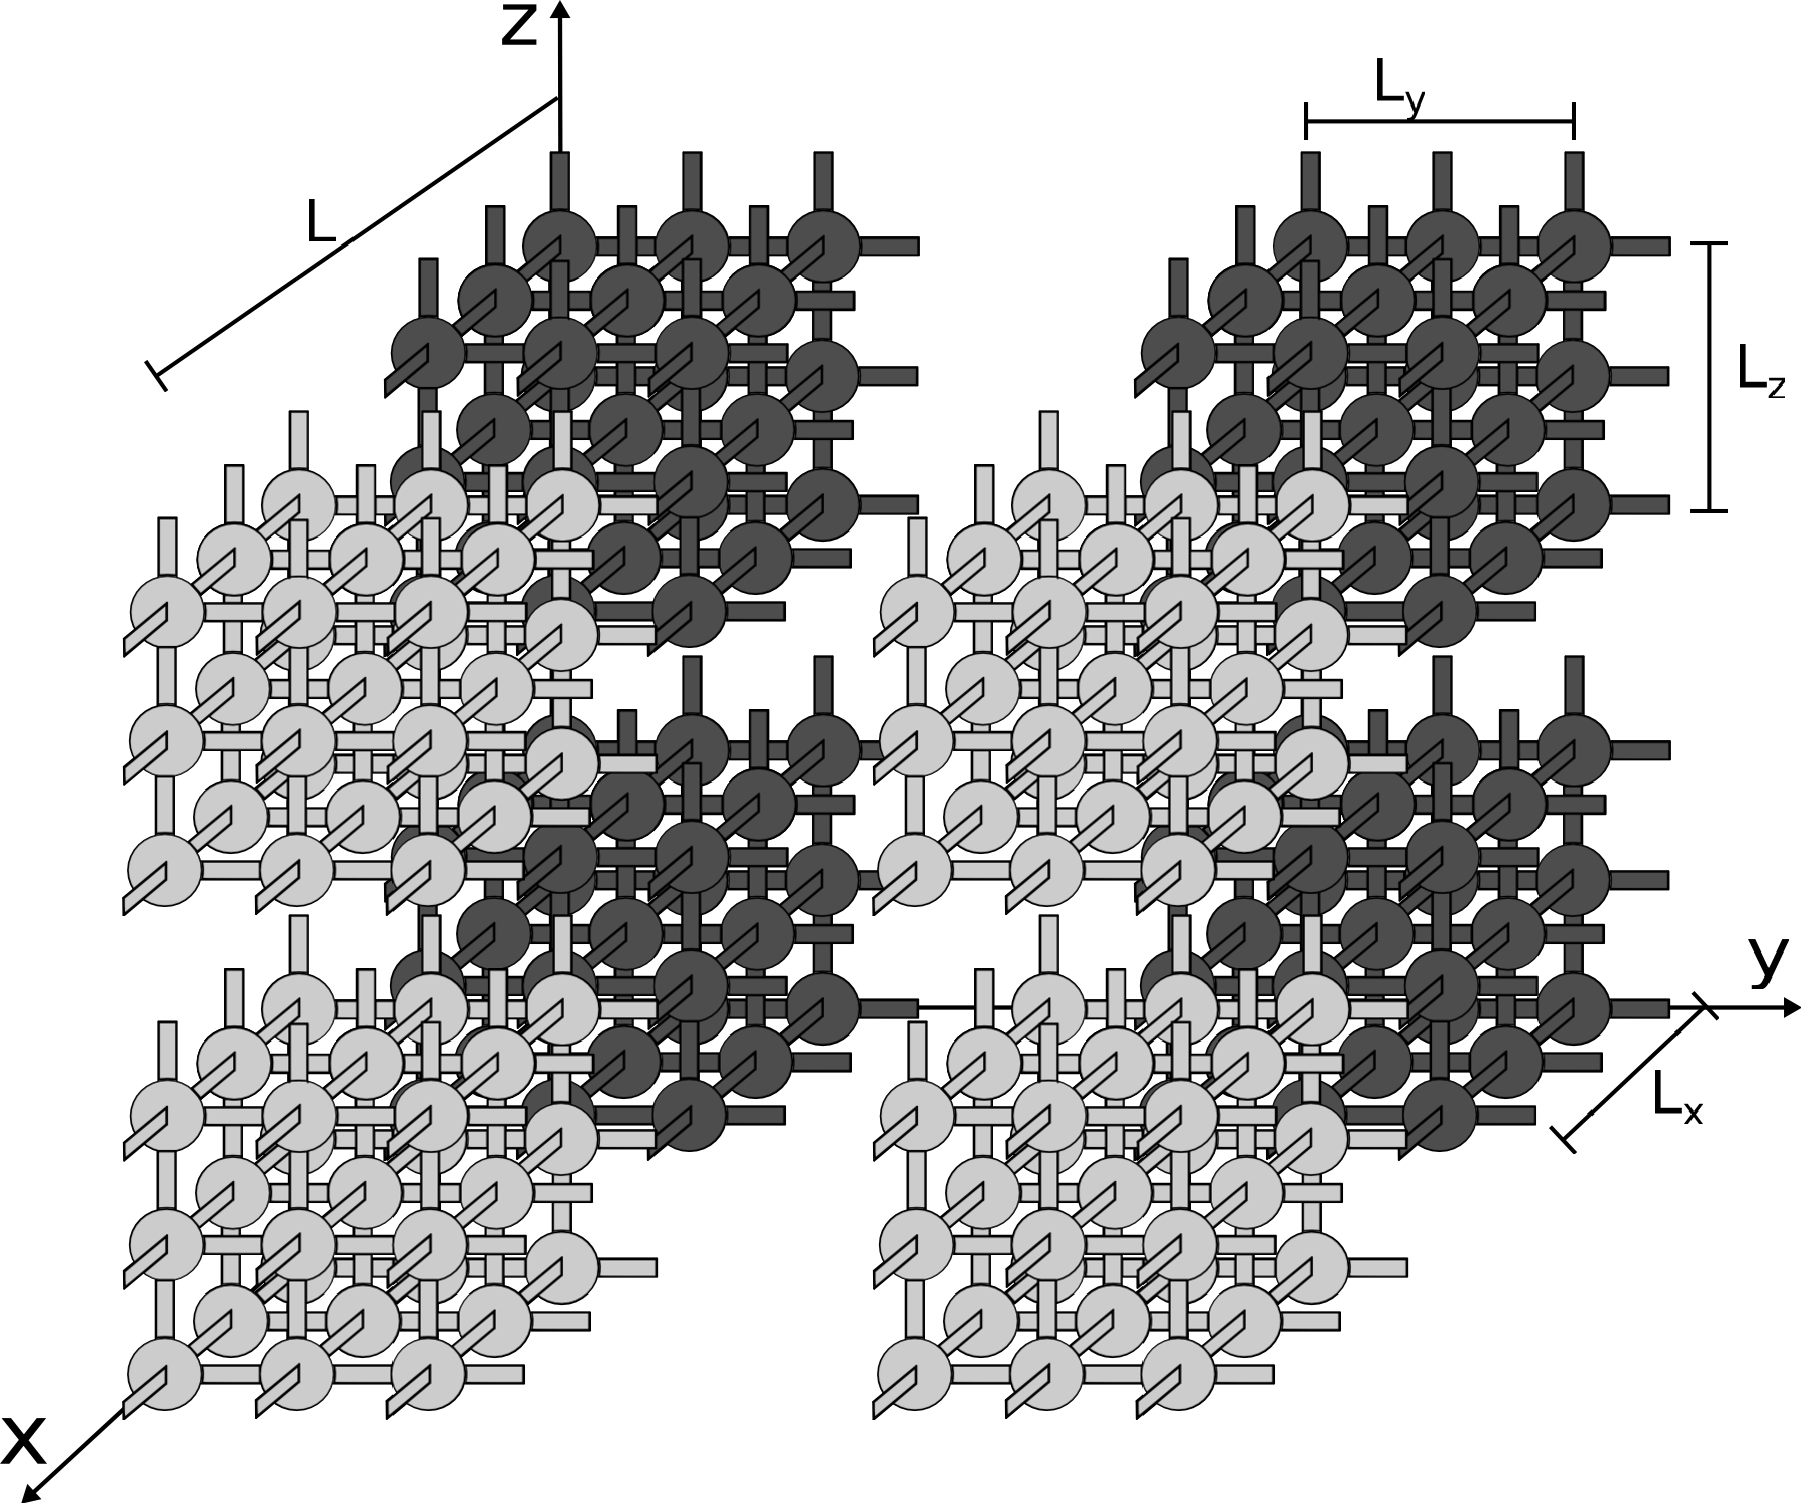
\includegraphics[width=3.5in]{img/distribucion.pdf}
\caption{Red porosa dividida en ocho subredes; $N=2\cdot2\cdot2$}
\label{fig:distribution}
\end{figure}

\begin{figure}[hbtp]
\centering
\begin{tabular}{cc}
\subfloat[$(1,2,2)$]{
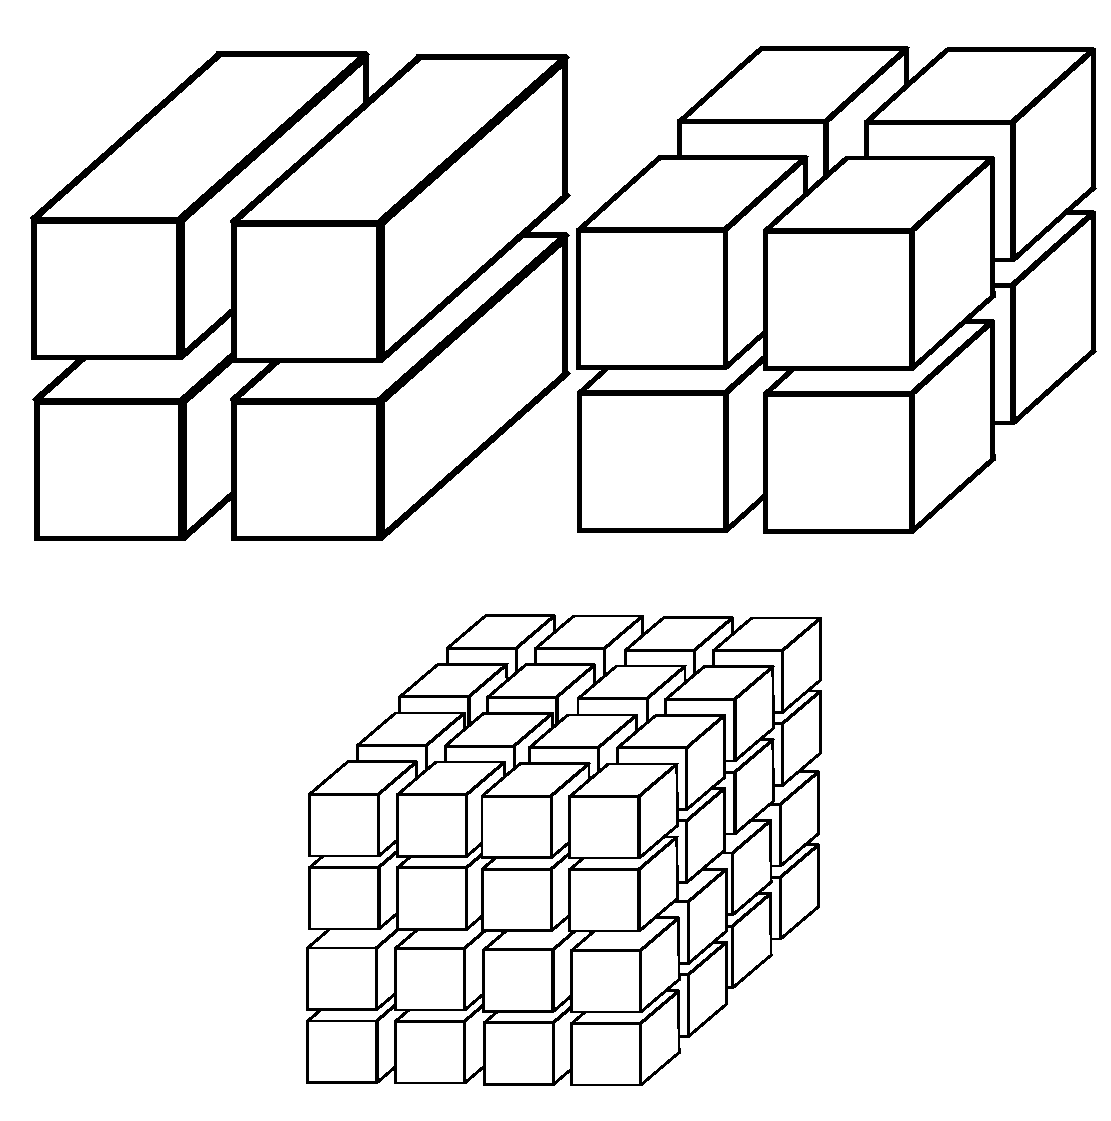
\includegraphics[width=2.0in, viewport=15 265 273 515,clip]
 {img/particionamiento.pdf}
\label{fig:part4}}
& \subfloat[$(2,2,2)$]{
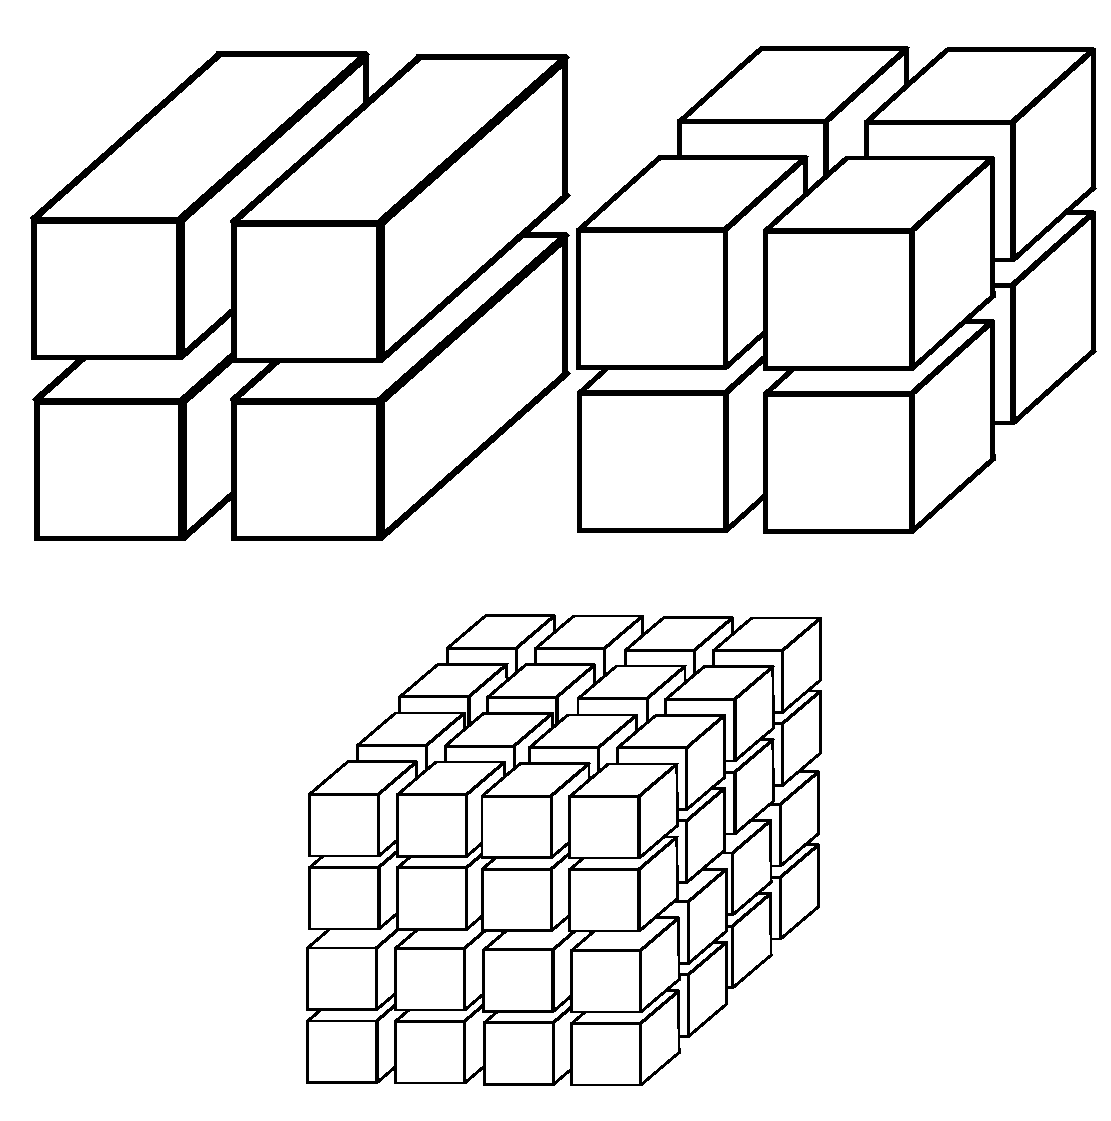
\includegraphics[width=2.0in, viewport=275 265 525 515,clip] {img/particionamiento.pdf}
\label{fig:part8}}\\

\multicolumn{2}{c}{
\subfloat[$(4,4,4)$]{
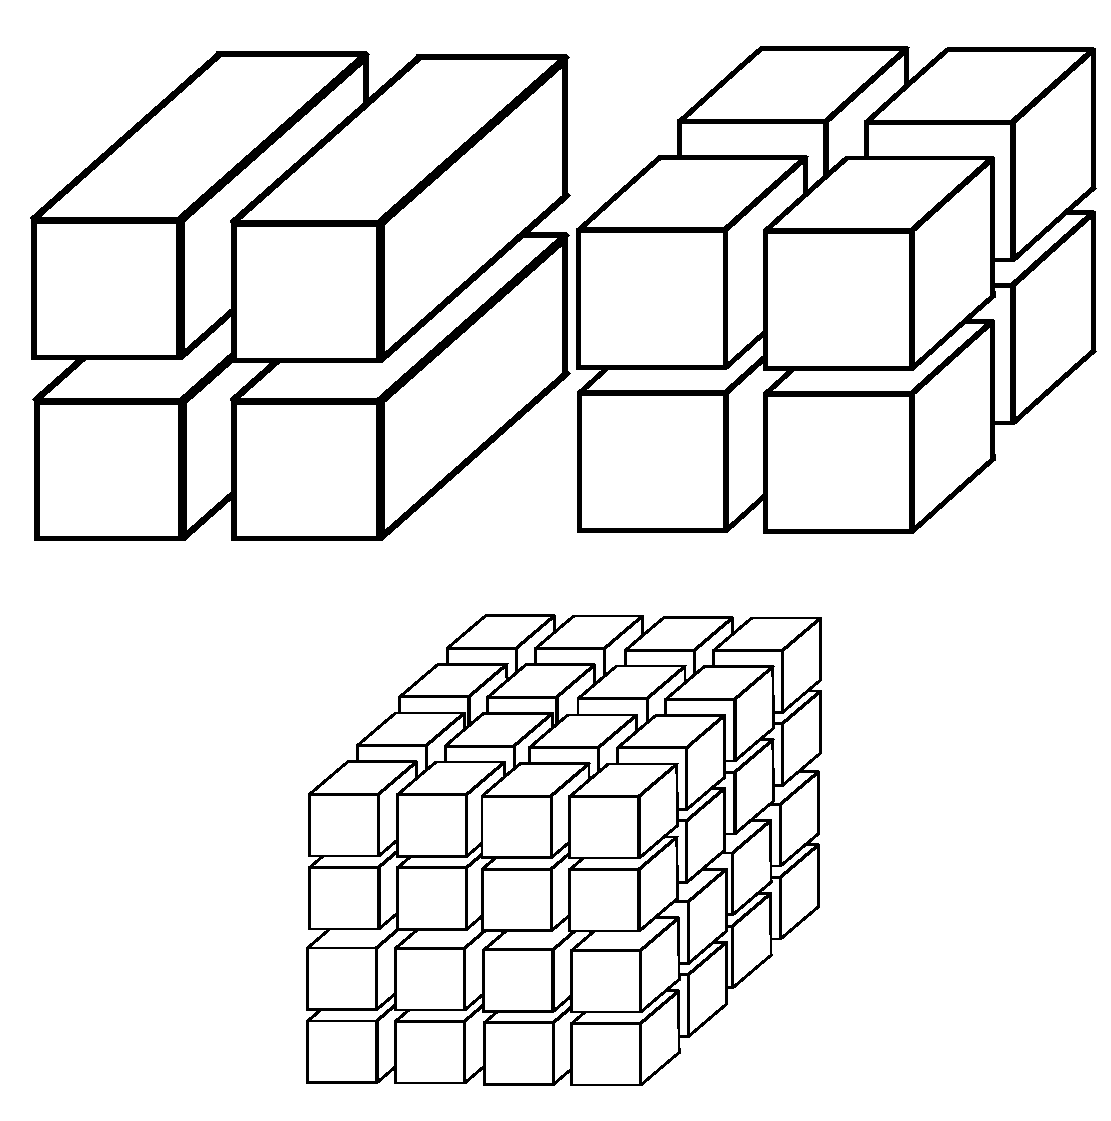
\includegraphics[width=2.0in, viewport=145 0 395 250,clip] {img/particionamiento.pdf}
\label{fig:part64}}
}
\end{tabular}

\caption{Distribución de la Red para (a) 4 hilos, (b) 8 hilos, and (c) 64 hilos}
\label{fig:particionamiento}
\end{figure}

Para permitir que la distribución del espacio de la red porosa no sea siempre el mismo, en este trabajo se propone
una distribución dinámica en donde el particionamiento no siempre empieza a partir del origen (0,0,0) de la red.
Se propone un cambio de origen con el propósito de obtener un desplazamiento lógico del espacio de la red, para que los hilos 
puedan trabajar en subredes independientes y diferentes de la red porosa.
En la Figura \ref{fig:shift} se muestra un red porosa distribuida a partir del origen (0,0,0) entre dos hilos (Figura \ref{fig:shift1}) 
y un ejemplo de un desplazamiento lógico sobre $y$, con cambio de origen a (0,2,0), puede verse en la Figura \ref{fig:shift1}. En esa figura
se observa que las subredes sobre las cuales 
trabajaran los hilos han cambiado, esta es una de las grandes ventajas de trabajar sobre memoria compartida ya que el tiempo 
que  toma un desplazamiento es totalmente despreciable ya que en ningún momento existe algún tipo de trasferencia física de los datos. 
Al contrario, si se utilizase memoria distribuida esta operación de desplazamiento se traduciría en trasferencia de 
datos entre nodos tal y como se comento en la Secci\'on \ref{subsec:algspar}, dicha trasferencia podría trasformarse en un cuello de botella.\\
\begin{figure}[hbtp]
\centering
\begin{tabular}{cc}
\subfloat[Distribución inicial]{
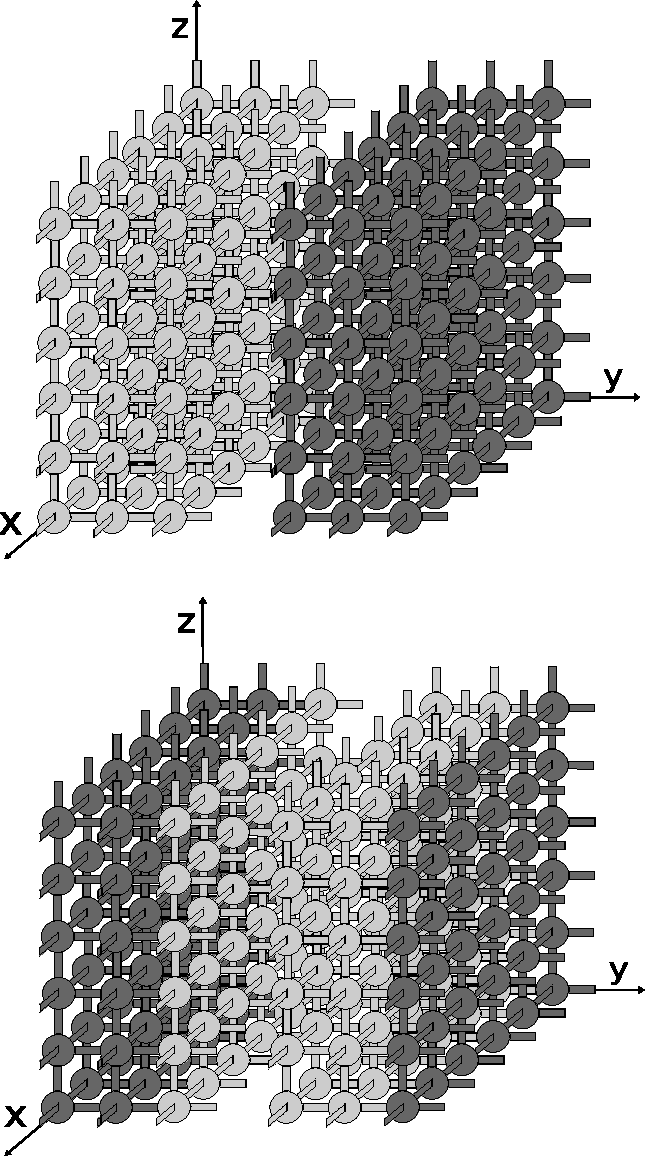
\includegraphics[width=2.5in, viewport=0  285 310 555,clip]{img/shift}
\label{fig:shift1}
}
& \subfloat[Desplazamiento sobre $y$]{
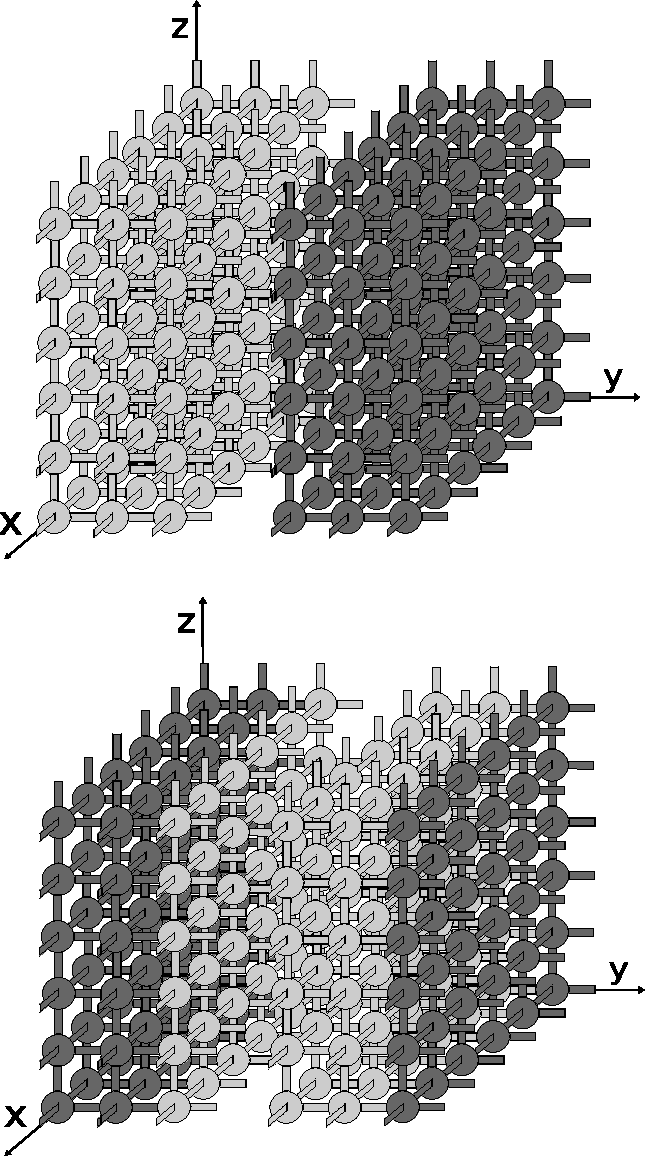
\includegraphics[width=2.5in, viewport=0 0 310 270,clip]{img/shift}
\label{fig:shift2}}
\end{tabular}
\caption{Ejemplo de un desplazamiento lógico (a) Posición inicial (0,0,0), (b) desplazamiento sobre $y$ (0,2,0)}
\label{fig:shift}
\end{figure}


\section{Solución Paralela Aleatoria basada en el Método de Monte Carlo}
\label{sec:pbiasedrg}
%\label{subsec:painit}
%\subsection{Inicialización}
%\label{subsec:painit}
Una vez que se determinó la distribución del espacio de la red porosa entre $N$ hilos como se presentó 
en la sección anterior, cada hilo trabaja de forma independiente en una de las subredes de tamaño $L_x \cdot L_y \cdot L_z$; 
la Figura \ref{fig:distribution} muestra un ejemplo de distribución de espacio poroso entre $8$ hilos.
En el proceso de inicializaci\'on cada hilo inserta de forma aleatoria en su subred $L_x \cdot L_y \cdot L_z$ sitios 
hasta rellenar por completo la red. Una vez que la red esta inicializada con sitios, a cada sitio se le asignan únicamente tres 
enlaces: izquierdo, trasero y superior. La asignación de dichos enlaces permite inicializar el contorno completo de cada
sitio, evitando la sincronización entre los hilos que accesan las caras externas de subredes adyacentes dentro de la red porosa global.

\subsection{Generación de una Red Porosa Válida}
\label{subsec:pbiasedrgvalid}
Después de que la red porosa ha sido inicializada ésta puede contener violaciones a las $RG$ ya que al igual que su 
respectiva versi\'on secuencial la inicializaci\'on no verifica el cumplimiento de las $RG$ al asignar un valor a los enlaces.
En seguida, para eliminar las violaciones se aplica una serie de $MCs$ Paralelos; este comportamiento se 
resume en el Algoritmo \ref{alg:pvalidnet}. Cada paso de $MC$ Paralelo implica que cada hilo 
aplicará un paso de $MC$ normal tal y como se hace 
en el algoritmo secuencial descrito en la secci\'on \ref{sec:svalid}, trabajando sobre su respectiva subred y omitiendo las caras 
externas (lineas 7-12 del Algoritmo \ref{alg:pvalidnet}). Al omitir las caras externas se evita la sincronizaci\'on entre hilos
que poseen subredes adyacentes.\\

Para que cada poro(sitio o enlace) de las caras externas de cada subred tenga la posibilidad de intercambiarse con otro, se realizan 
desplazamientos lógicos a lo largo de los ejes $x$, $y$ y $z$ después de ejecutar cada paso de $MC$ 
Paralelo(linea 17 del algoritmo \ref{alg:pvalidnet}).
Con dichos desplazamientos se logra que caras externas en un momento queden al interior de una subred. Al igual que en la versi\'on 
secuencial los pasos de $MC$ Paralelos se repetirán hasta eliminar por completo las violaciones a las $RG$.\\

\begin{algorithm}
\caption{Algoritmo paralelo de $MC$ para generar una red porosa válida}\label{alg:pvalidnet}
\begin{algorithmic}[1]
\algblockdefx[NAME]{ompparallel}{eompparallel}
    {\textbf{omp parallel private $(tid,nMCs,exchanges)$}}
    {\textbf{end omp parallel}}    
\algblockdefx[NAME2]{ompmaster}{eompmaster}
    {\textbf{omp master}}
    {\textbf{end omp master}}
\Require $pnet$: red porosa
\Require $dist$: Arreglo con la distribución de la red
\State $continue \gets$ \Call{GRviolations}{$\&pnet$} $ > 0$
\ompparallel
	\State $tid \gets $ \Call{OmpGetTid}{ }
	\State $nMCs=4(( dist[tid].L_x  - 2) \cdot (dist[tid].L_y - 2) \cdot (dist[tid].L_z - 2))^3$
	\While{$continue$}
		\State $exchanges \gets nMCs$
		\While{$(exchanges--)> 0$}
			\State \Call{PoreExchange}{$\&pnet,\&dist[tid]$}
			\If{\Call{NonValidExchange}{$\&pnet,\&dist[tid]$}}
				\State \Call{RejectExchange}{$pnet,dist[tid]$}
			\EndIf
		\EndWhile
		
		\State \textbf{omp barrier}
		
		\ompmaster
			\State $continue \gets$ \Call{GRviolations}{$\&pnet$} $ > 0$		
			\If{$continue$}
				\State \Call{Shift}{$\&pnet,\&dist[tid]$} {$//$ desplazamiento sobre ($x,y,z$)}
			\EndIf
		\eompmaster

		\State \textbf{omp barrier}
	\EndWhile
\eompparallel
\end{algorithmic}
\end{algorithm}

\section{Solución Paralela Híbrida}
\label{sec:ph}
A continuación describiremos el algoritmo paralelo correspondiente al algoritmo secuencial descrito en la secci\'on \ref{sec:hybrid}. Al 
igual que en su versi\'on secuencial el algoritmo presentado en esta secci\'on se compone de 3 principales pasos: inicalizaci\'on (sembrado 
de clusters de sitios y asignación de enlaces), generación de una red porsa v\'alida y mejoramiento de isotropía. El algoritmo hace uso 
del algoritmo de distribución dinámica descrito en la sección \ref{sec:pdistribution} para distribuir la red porsa entre los $N$ hilos 
a utilizar. Cada hilo ejecuta en paralelo la etapa de inicilización, luego  se aplican sucesivos pasos de $MC$ paralelos para eliminar 
las violaciones a las $RG$. Al finalizar el algoritmo obtiene una red porosa libre de violaciones a las $RG$.

\subsection{Inicialización}
\label{subsec:pinit}
Igual que en el algoritmo basado en Monte Carlo, en esta versión Híbrida los hilos trabajan en subredes diferentes. 
En la inicialización cada hilo genera dos listas ordenadas $L_S$ y $L_B$, también se crea la lista $L_{SC}$ la cual inicialmente estará vacía. 
$L_S$ contiene $L'$ elementos de tamaños de sitos ordenados de forma descendente, y $L_B$ contiene $3L'$ elementos de tamaños de enlaces 
ordenados también de forma descendente, donde $L'$ es igual a $L_x \cdot L_y \cdot L_z$. Cabe destacar que $L'$ es local a cada hilo 
ya que aun cuando el algoritmo de distribución de la red intenta que las subredes sean del mismo tamaño, existen casos en los cuales 
no es posible, ésto da como resultado subredes de diferentes tamaños. La sincronización entre los hilos no es necesaria para 
el uso o modificación de las listas $L_S$, $L_{SC}$ y $L_B$ porque estas listas son locales a cada hilo.

\subsubsection{Sembrado de Clusters y Rellenado de la Red Porosa}
\label{subsec:pseeding}
Por cada hilo, el número de semillas corresponde a $NClusters/N$. Cada semilla es insertada en una posición aleatoria en su 
respectiva subred. Los demás elementos en $L_S$ son tomados uno por uno para cubrir la semilla y formar un cluster, tal y como se 
explica en el capítulo anterior. La posición aleatoria en la cual se asignará la semilla en la subred es generada de tal forma 
que no puede ser asignada en las caras externas de la subred. Durante el sembrado todos los hilos se sincronizan a través 
de una $barrera$ después de que cada uno complete un cluster, entonces el origen $(x, y, z)$ de distribución se desplaza 
de forma aleatoria a lo largo de los ejes $x$,$y$ y $z$ en un rango que esta entre $0$ y $L-1$. 
El cambio de origen de distribución nos ayuda a que cada hilo tenga la posibilidad de sembrar un cluster en cualquier 
posición de la red porosa.\\

El la Figura \ref{fig:origin} se muestra un ejemplo del cambio de origen durante el proceso de sembrado. La Figura \ref{fig:origin1} 
muestra dos clusters de sitios construidos al tener el origen de la red porosa inicialmente en $(0,0,0)$. Si movemos el origen a $(0,L/2,0)$, 
esto causaría que las áreas de trabajo(subredes) de cada hilo cambien para construir en paralelo otro cluster de sitios, 
como se muestra en la Figura \ref{fig:origin2}. Las áreas de trabajo de cada hilo se resaltan en color azul y naranja, antes y después
del desplazamiento. El cambio de origen, adem\'as de permitir que las caras externas de cada subred sean tomadas en 
cuenta durante el sembrado, nos permite hacer parecer(emular) que la red porosa fue inicializada por un solo hilo como en la versión secuencial,
ya que prácticamente cada hilo podría trabajar en algún momento en cualquier parte de la red porosa.\\

\begin{figure}[hbtp]
\centering
\begin{tabular}{c}

\subfloat[Distribución inicial del espacio]{
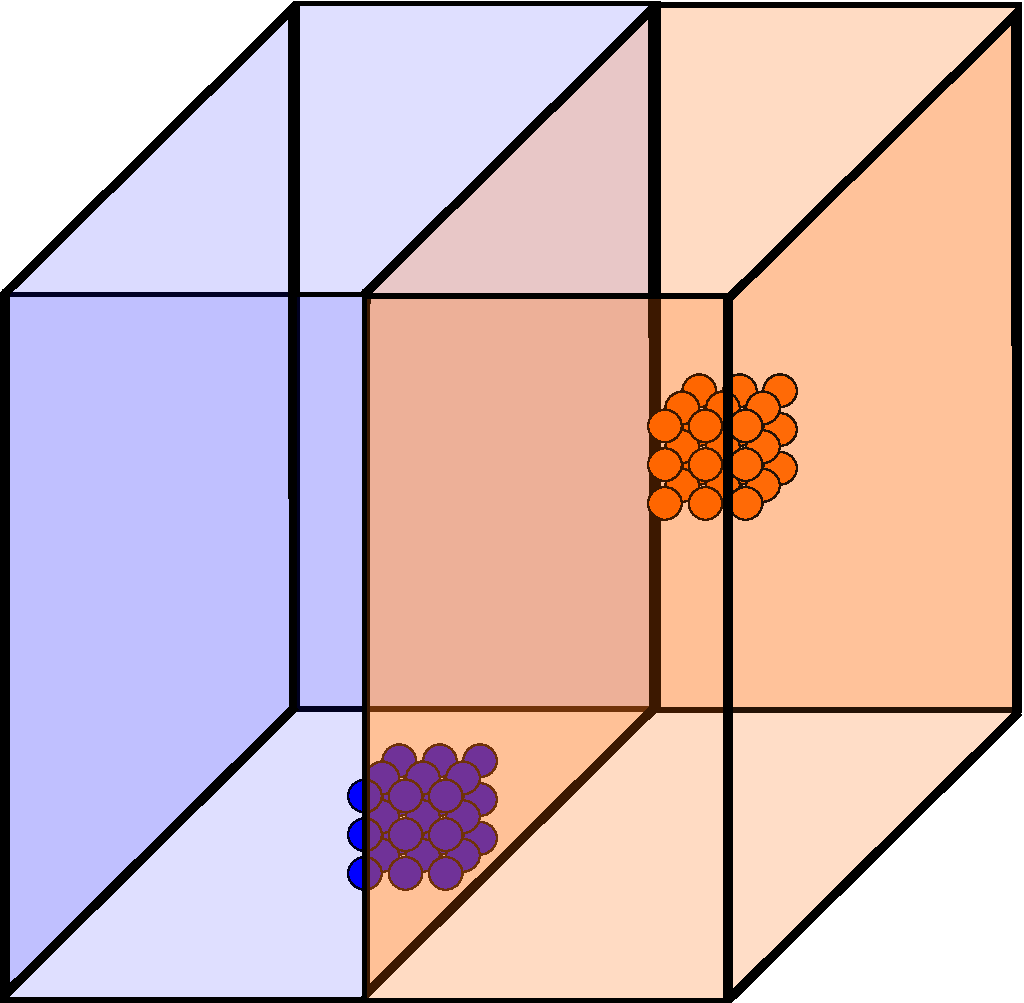
\includegraphics[width=4.0in]{img/origin1.pdf}
\label{fig:origin1}}\\

\subfloat[Distribución posterior del espacio]{
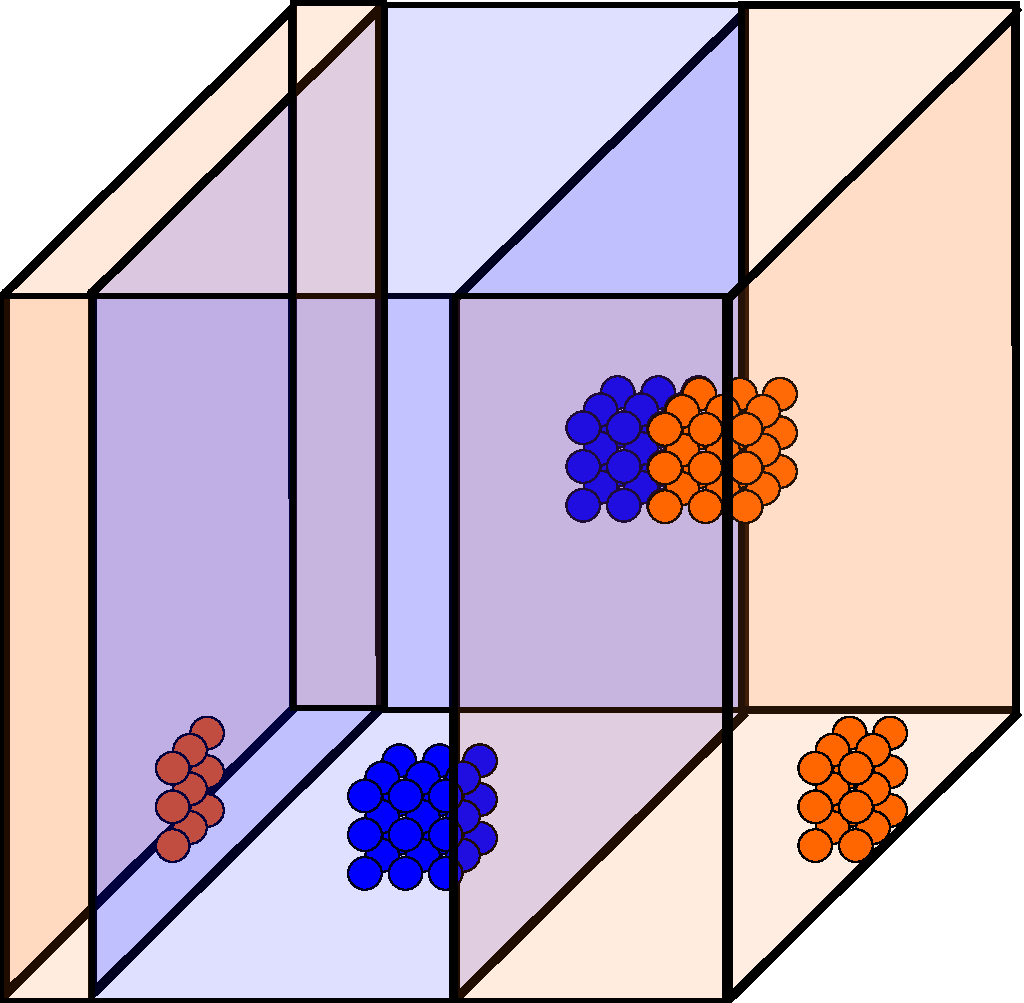
\includegraphics[width=4.0in] {img/origin2.pdf}
\label{fig:origin2}}

\end{tabular}

\caption{(a) Origen en ($0,0,0$) y (b) cambio de origen a ($0,L/2,0$)}
\label{fig:origin}
\end{figure}

Después de completar el sembrado de clusters, el origen de la red es trasladado a ($0, 0, 0$) de manera que cada hilo
comienza a trabajar en su subred inicial. El siguiente paso consiste en rellenar su actual subred con los sitios restantes 
en su lista $L_S$; sin embargo, debido a posibles translapes durante el sembrado de clusters, en este momento el número 
de sitios en las listas $L_S$ de cada hilo es diferente. Puede ser que para algunos hilos los sitios que tienen en sus 
listas $L_S$ no sean suficientes para rellenar su subred, mientras que para otros el número de sitios en sus listas $L_S$ puede 
ser mayor al de los requeridos para rellenar su subred. Para solucionar este problema los elementos de las listas $L_S$ 
requieren ser distribuidos entre los hilos.\\

Los pasos necesarios para distribuir los elementos de las listas $L_S$ se presentan en el Algoritmo \ref{alg:sitesdist} el 
cual es una versión simplificada del algoritmo presentado en \cite{ref11} para la distribución de carga.\\
Por cada hilo se tiene, identificador del hilo ($id$), el número $M[id]$ de sitios requeridos el cual depende de: el tamaño 
de la subred $SNS[id]$ ($SNS[id] = L_x \cdot L_y \cdot L_z$), el número de sitios que ya han sido insertados en la subred $SI[id]$, 
y el número de sitios en su lista $AL_S[id]$, denotado por $Size(L_S[id])$. En el algoritmo el arreglo $M$ tiene contexto global 
por lo cual es una variable compartida.\\

La primera etapa consiste en el calculo del número de sitios requeridos; cada hilo calcula $M[id]$ como se indica en la linea 
1 del Algoritmo \ref{alg:sitesdist}. En el segundo paso, los hilos que tienen $M[id]<0$ (los que tienen sitios de 
sobra) insertan su $id$ en la lista compartida de Hilos Pesados denotada por $HT$,(line 4). Esta inserción 
se hace a través de exclusión mutua entre los hilos (lineas 2-6). Después todos los hilos se sincronizan mediante un 
mecanismo de barrera (linea 7). Esta barrera hace que los hilos con $M[id]>0$ (con sitios faltantes) esperen a que 
la lista $HT$ sea inicializada por los demás hilos. En el último paso, los hilos con $M[id] > 0$ trabajan utilizando 
exclusión mutua (lineas 9-23) para tomar sus sitios faltantes de las listas $L_S$ de los hilos en $HT$. Cuando un hilo $id$ 
toma los sitios de otro hilo $k$ en $HT$ (lineas 13 y 17), los nuevos valores $M[id]$ y $M[k]$ se actualizan, como se 
muestra en las lineas 14, 15, 18 y 19. En caso de que un hilo en $HT$ había dado todos sus sitios sobrantes, éste es removido 
de la lista $HT$ (linea 20).\\

Una vez que la distribución de los sitios es completada, cada hilo hace crecer su primer cluster generado hasta rellenar por 
completo su subred y su lista $L_S$ queda vacía.
 
%\newcommand{\INDSTATE}[1][1]{\State\hspace{#1\algorithmicindent}}
\begin{algorithm}
\caption{Algoritmo de redistribución de los sitos entre los hilos}\label{alg:sitesdist}
\begin{algorithmic}[1]
%\algblock[Name]{ompcritical}{End}
\algblockdefx[NAME]{ompcritical}{eompcritical}
    {\textbf{omp critical}}
    {\textbf{end omp critical}}
    
\Require $M$: Arreglo compartido
\Require $HT$: Lista compartida de hilos pesados
\Require $id$: Identificador del hilo
\State $M[id]=SNS[id]-SI[id]-Size(L_S[id])$
\If{$M[id]<0$}
	\ompcritical
		\State \Call{InsertId}{$id,HT$}
	\eompcritical
\EndIf
\State \textbf{omp barrier}
\If{$M[id]>0$}
	\ompcritical
		\While{$M[id] > 0$}
			\State $k=getFirst(HT)$
			\If{$M[id] < |M[k]| $}
				\State \Call{MoveNSites}{$M[id],L_S[id],L_S[k]$}
				\State $M[k]=M[k]+M[id]$
				\State $M[id]=0$
			\Else
				\State \Call{MoveNSites}{$M[k],L_S[id],L_S[k]$}
				\State $M[k]=0$
				\State $M[id]=M[id]+M[k]$
				\State \Call{RemoveId}{$k,HT$}	
			\EndIf
		\EndWhile
	\eompcritical
\EndIf
\end{algorithmic}
\end{algorithm}

\subsubsection{Asignación de Enlaces}
\label{subsec:pbond}
En la parte del sembrado de clusters de sitios cada hilo también mantuvo su lista $L_{SC}$ del mismo modo que se hace en la versión secuencial.
La listas $L_{SC}$ de cada hilo contienen las posiciones en las cuales se insertaron los sitios a lo largo de la red porosa; sin embargo 
los elementos de cada lista $L_{SC}$ están dispersos en todo el espacio de la red porosa.\\

Debido a las acciones realizadas en la sección anterior las listas $L_{SC}$ pueden estar en desbalance, por lo que es necesario 
distribuir los elementos entre los hilos. Para distribuir los elementos de las listas $L_{SC}$ se utiliza el mismo algoritmo de 
la sección anterior (Algoritmo \ref{alg:sitesdist}), con dos cambios. El primer cambio sustituye en todo el algoritmo $L_S$ por 
$L_{SC}$ y el segundo cambia la linea 1 por $M[id]=SNS[id]-Size(L_{SC}[id])$.\\

Una vez que las listas están balanceadas, cada hilo, toma las posiciones de los sitos una a uno de la lista $L_{SC}$ y conecta los 
tres correspondientes enlaces al sitio (izquierdo, trasero y superior). Cada conexión entre sitio y enlace debe cumplir con 
el $PC$ y las $RG$, siguiendo el mismo procedimiento descrito en la sección \ref{subsec:sbonds}. Cada sitio es conectado a 
solo tres enlaces porque, como se define en el Capítulo \ref{champ:intro}, un sitio tiene tres enlaces propios mientras que 
los otros tres enlaces son compartidos con los sitios vecinos. Lo anterior se hace para evitar la sincronización entre los 
hilos que posiblemente se necesitaría al conectar los enlaces compartidos (derecho, frontal e inferior). Al finalizar este 
paso se obtiene una red porosa con posibles violaciones al $PC$ y a las $RG$.

\subsection{Generación de una red porosa válida}
\label{subsec:pvalid}
Para que la red creada a partir de los pasos descritos en las secciones anteriores sea válida en términos del $PC$ y de 
las $RG$, es necesario aplicar una serie de pasos de $MC$ Paralelos Modificados ($MMC$-Paralelos). $MMC$-Paralelos se basa
 en los $MCs$ Paralelos utilizados en la Secci\'on \ref{subsec:pbiasedrgvalid} 
con dos grandes modificaciones. La primer modificación es que se utiliza la operación de cambio de origen y la segunda es que a cada hilo 
se le asignan dos subredes. Ambas modificaciones fueron pensadas para que, al igual que un paso de $MC$ normal, cada poro pueda 
ser intercambiado por cualquier otro de la red porosa. Por cada intercambio de sitios o enlaces durante un $MMCs$ se verifica 
que se cumpla tanto con el $PC$ y las $RG$. A continuación se detallan los pasos para la eliminación de las violaciones a las $RG$:

\begin{enumerate}
\item La red porosa es dividida en $2N$ subredes como se describe en la Sección \ref{sec:pdistribution}.

\item A cada hilo se le asignan aleatoriamente dos subredes de las generadas en el paso anterior

\item Los intercambios se omiten si los poros involucrados pertenecen a las caras  externas de sus subredes

\item Cada hilo genera una lista $L_{SE}$ que contiene las posiciones de los sitios que no cumplen con las $GR$ en ambas subredes asignadas 

\item Si $Size(L_{SE}) > 0$, se toma el primer elementos de la lista $L_{SE}$ que es la posición de un sitio con violaciones geométricas, 
en otro caso se toma aleatoriamente la posición de un sitio de cualquiera de las dos subredes asignadas, esta posición se 
etiqueta como $s1$. Una posición($s2$) de un sitio se toma aleatoriamente de cualquiera de las dos subredes asignadas. Posteriormente, 
$s1$ y $s2$ se intercambian mutuamente sitios o enlaces (ej. intercambiar el enlace derecho de $s1$ por el enlace frontal de $s2$). El 
intercambio se mantiene solo si el número de violaciones a las $RG$ es menor o igual al número de violaciones antes del intercambio, en 
otro caso el intercambio es rechazado

\item El paso 5 se repite $4(( L_x  - 2) \cdot (L_y - 2) \cdot (L_z - 2))^3$ veces por cada hilo, después de esto el origen de la red 
se desplaza de forma aleatoria para que los hilos puedan trabajar en regiones distintas de la red a las que inicialmente se les asignaron

\item Cada hilo calcula el número total de sitios con violaciones a las $GR$ en ambas subredes, de existir , incluyendo las caras 
externas. Cuando el número total de violaciones es igual a cero el algoritmo termina, en otro caso se repite desde el paso 4
\end{enumerate}

\section{Mejoramiento de la isotropía}
\label{subsec:pisotropy}
Para mejorar la isotropía es necesario aplicar un numero adicional ($K$) de pasos de $MMC$-Paralelos para las redes creadas ya sea por 
el algoritmo de la Sección \ref{sec:pbiasedrg} o el algoritmo de la Sección \ref{sec:ph} respectivamente. En el primer caso se sigue 
el mismo procedimiento del algoritmo descrito en la Secci\'on \ref{subsec:pbiasedrgvalid} y en el segundo se sigue el procedimiento 
descrito en la Sección \ref{subsec:pvalid}, ambos procedimientos se deben de repetir $K$ veces.